\section{Site Internet}
Pour commencer, vous pouvez trouver notre site web à l'adresse suivante : cmalt-ocr.epiproject.eu.\\
Pour ce site, nous avons décidé de faire une interface simple, épuré et pas très rechercher pour facilité la navigation. Pour cela, nous avons utilisé du HTML/CSS et du PHP. Notre site est hébergé sur le serveur de de Louis Forget.\\
Le site internet n'est pas une partie principale du projet, il passe souvent au second plan à cause des difficultés rencontré au cours du projet. Cependant, nous avons fait en sorte que notre site ne soit pas délaissé.

\subsection{HTML/CSS}
La base de notre site repose sur le language HTML (HyperText Markup Language) qui gère et organise le contenu. Vous direz par exemple : « Ceci est mon titre, ceci est mon menu, voici le texte principal de la page, voici une image à afficher, etc. » et il vous l'afichera dans une page comme indiqué dans votre code. Cependant, il ne fera qu'afficher, sans aucun style ni mise en page, des paragraphes et des titres écrit en noir sur fond blanc. C'est là qu'intervient le CSS (Cascading Style Sheets, aussi appelées Feuilles de style) qui va révlutionner la page que vous êtes en train de créer. Le rôle du CSS est de gérer l'apparence de la page (agencement, positionnement, décoration, couleurs, taille du texte…) Ce qui va donner une ame à votre site (sauf s'il est roux, mais j'en doute...).\\

C'est ainsi que notre site a vu le jour, mais il a falu l'amélioré, et la, un autre problème s'est posé, comme chaque page du site a le même squelette, modifier une toute petite partie de celui ci revient à modifier à la main chaque page du site, ce qui n'est pas très sypatique pour aller vite. Mais nous avons trouvé la solution, nous avons introduit du PHP dans notre code !

\subsection{PHP}
Le PHP est un langage que seuls les serveurs comprennent et qui permet de rendre les sites dynamiques. C'est PHP qui « génère » la page web. Une de ces principals fonction est de "se souvenir" des bouts de code (c'est pas pour rien que c'est un éléphant). En effet, pour que notre site est le même squelette sur toute ses pages, nous allons écrire un squelette dans un fichier et nous utiliserons une balise PHP pour le "charger" dans toute les page de notre site. Grâce à se procédé miraculeux, nous pouvons modifier le squelette du site tout entier en ne modifiant qu'un seul fichier. Bien enttendu notre site ne comporte pas beaucoup de pages, mais nous utilisons cette methode pour éviter les pages anciennes au milieu des nouvelles.


\begin{figure}[h]
  \begin{center}
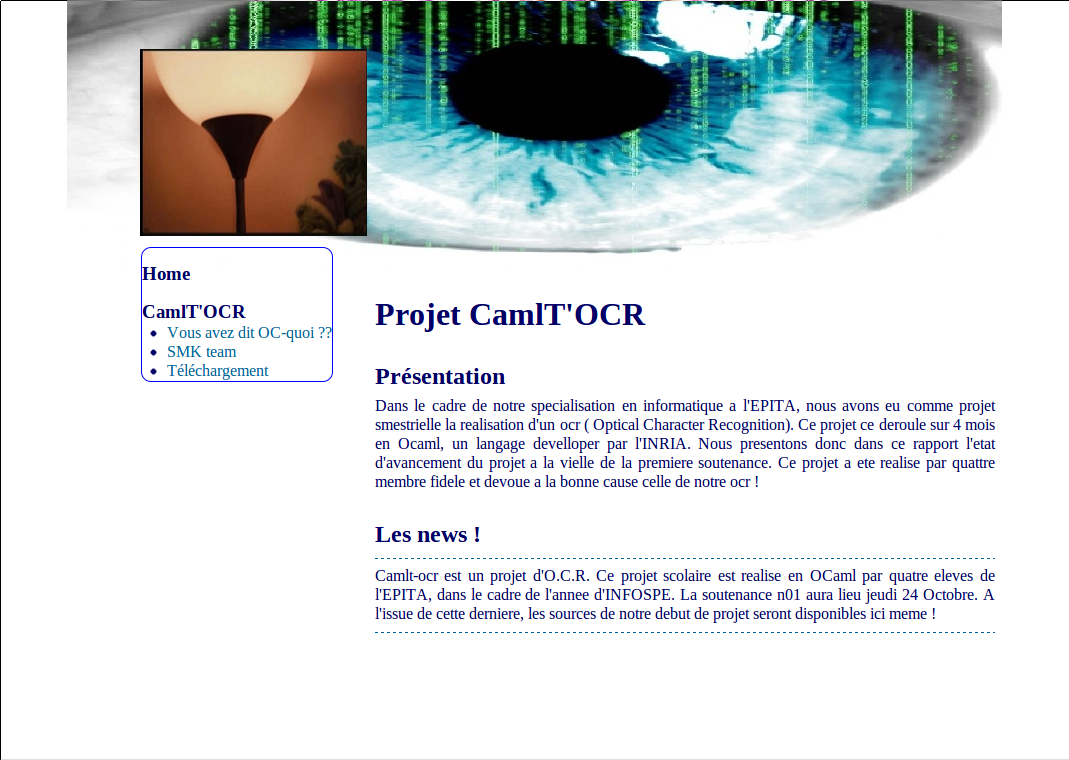
\includegraphics[width=0.50\textwidth]{site.png}
\caption{la page principale du site internet}
\end{center}
\end{figure}